% docs/slides/preamble.tex -- 五份 deck 共享
\documentclass[aspectratio=169,11pt]{beamer}

% ==== 中文与字体 ====
\usepackage[UTF8,fontset=none]{ctex}
\usepackage{fontspec}

\IfFontExistsTF{PingFang SC}{%
  \setCJKmainfont{PingFang SC}[BoldFont=PingFang SC,ItalicFont=PingFang SC,AutoFakeSlant=0.15]
  \setCJKsansfont{PingFang SC}[ItalicFont=PingFang SC,AutoFakeSlant=0.15]
  \setCJKmonofont{PingFang SC}
}{%
  \IfFontExistsTF{Source Han Sans SC}{%
    \setCJKmainfont{Source Han Sans SC}
    \setCJKsansfont{Source Han Sans SC}
  }{%
    \IfFontExistsTF{Noto Sans CJK SC}{%
      \setCJKmainfont{Noto Sans CJK SC}
      \setCJKsansfont{Noto Sans CJK SC}
    }{%
      \setCJKmainfont{Heiti SC}
      \setCJKsansfont{Heiti SC}
    }
  }
}

\IfFontExistsTF{Helvetica Neue}{\setmainfont{Helvetica Neue}}{%
  \IfFontExistsTF{Inter}{\setmainfont{Inter}}{}}
\IfFontExistsTF{JetBrains Mono}{\setmonofont{JetBrains Mono}[Scale=0.85]}%
  {\setmonofont{Menlo}[Scale=0.85]}

% ==== 颜色 ====
\usepackage{xcolor}
\definecolor{cMain}{HTML}{1F4E79}
\definecolor{cAccent}{HTML}{E07A1F}
\definecolor{cGray}{HTML}{595959}
\definecolor{cMute}{HTML}{F4F4F4}
\definecolor{cOK}{HTML}{2E7D32}
\definecolor{cBad}{HTML}{B23A3A}
\definecolor{cWarn}{HTML}{C8A300}

% ==== 主题 ====
\usepackage{tcolorbox}
\usetheme{metropolis}
\metroset{progressbar=frametitle,numbering=fraction,block=fill}
\setbeamercolor{frametitle}{bg=cMain,fg=white}
\setbeamercolor{progress bar}{fg=cAccent,bg=cMute}
\setbeamercolor{alerted text}{fg=cAccent}
\setbeamercolor{title}{fg=cMain}

% metropolis 默认尝试 Fira Sans，未安装时 fallback 到 Latin Modern Sans。
% 这里在主题加载后显式覆盖，强制使用 macOS 上一定存在的 Helvetica Neue，
% 跟中文 PingFang 风格一致；找不到则按顺序尝试 Inter / Arial。
\IfFontExistsTF{Helvetica Neue}{%
  \setsansfont{Helvetica Neue}%
}{%
  \IfFontExistsTF{Inter}{\setsansfont{Inter}}{%
    \IfFontExistsTF{Arial}{\setsansfont{Arial}}{}}%
}

% ==== TikZ ====
\usepackage{tikz}
\usetikzlibrary{positioning,arrows.meta,fit,shapes.geometric,calc,%
  decorations.pathmorphing,backgrounds}

\tikzset{
  node-box/.style={draw=cMain,thick,rounded corners=2pt,
    minimum height=8mm,minimum width=18mm,align=center,font=\small},
  node-state/.style={draw=cMain,thick,circle,minimum size=14mm,
    align=center,font=\small},
  node-ok/.style={draw=cOK,thick,fill=cOK!10},
  node-warn/.style={draw=cWarn,thick,fill=cWarn!15},
  node-bad/.style={draw=cBad,thick,fill=cBad!10},
  % 色盲友好的状态机三态：蓝 (正常/Closed) / 橙 (告警/Open) / 灰 (中间/HalfOpen)
  % 避免 red-green 二元区分，改用 hue + lightness 双通道。
  node-state-normal/.style={draw=cMain,thick,fill=cMain!12},
  node-state-alert/.style={draw=cAccent,thick,fill=cAccent!18},
  node-state-transition/.style={draw=cGray,thick,fill=cGray!18},
  arrow/.style={-{Stealth[length=2mm]},thick,draw=cMain},
  arrow-async/.style={-{Stealth[length=2mm]},thick,dashed,draw=cGray},
  arrow-bad/.style={-{Stealth[length=2mm]},thick,draw=cBad},
  arrow-alert/.style={-{Stealth[length=2mm]},thick,draw=cAccent},
  lifeline/.style={dashed,thick,draw=cGray},
}

% ==== 代码 ====
\usepackage{listings}
\lstdefinelanguage{Go}{
  morekeywords={break,case,chan,const,continue,default,defer,else,
    fallthrough,for,func,go,goto,if,import,interface,map,package,range,
    return,select,struct,switch,type,var,nil,true,false,iota},
  morekeywords=[2]{string,int,int64,uint,uint64,bool,byte,error,context},
  sensitive=true,
  morecomment=[l]//,morecomment=[s]{/*}{*/},
  morestring=[b]",morestring=[b]`,
}
\lstdefinelanguage{LuaRedis}{
  morekeywords={and,break,do,else,elseif,end,false,for,function,if,in,
    local,nil,not,or,repeat,return,then,true,until,while},
  morekeywords=[2]{redis,call,KEYS,ARGV,tonumber,HGET,HSET,GET,SET,
    DECR,DECRBY,INCR,INCRBY,EXPIRE,PEXPIRE,ZADD,ZCARD,ZREMRANGEBYSCORE,
    EVAL,EVALSHA},
  sensitive=true,
  morecomment=[l]{--},
  morestring=[b]",morestring=[b]',
}

\lstdefinestyle{base}{
  basicstyle=\ttfamily\scriptsize,
  numbers=left,numberstyle=\tiny\color{cGray},
  keywordstyle=\color{cMain}\bfseries,
  keywordstyle=[2]\color{cAccent},
  stringstyle=\color{cOK},
  commentstyle=\color{cGray}\itshape,
  backgroundcolor=\color{cMute},
  frame=single,framerule=0pt,
  showstringspaces=false,
  breaklines=true,
  tabsize=2,
  columns=fullflexible,
}
\lstset{style=base}

% ==== 三线表与附录页码 ====
\usepackage{booktabs}
\usepackage{appendixnumberbeamer}

% ==== 页脚来源标注 ====
\newcommand{\srcnote}[1]{{\color{cGray}\scriptsize\itshape #1}}

% 关键论点框
\newcommand{\keypoint}[1]{%
  \begin{tcolorbox}[colback=cMute,colframe=cMain,boxrule=0.5pt,arc=2pt]%
  #1\end{tcolorbox}}


\title{商家后台与可观测性（v2 扩展版）}
\subtitle{从五角色视角看一个商家入驻 / 一次客诉定位 / 一笔退款 / 一次大促 SLO 守护}
\author{gomall · 业务侧 deck}
\date{}

\begin{document}

\maketitle

\begin{frame}{今日大纲}
\tableofcontents
\end{frame}

% ============================================================
\section{业务视角先行：商家后台 + 可观测对谁有什么用}
% ============================================================

\begin{frame}{五个角色，五个截然不同的问题}
\begin{tikzpicture}[node distance=3mm and 7mm,every node/.append style={align=center,font=\scriptsize,text width=28mm,minimum height=14mm}]
  \node[node-box,node-state-normal]                  (c)   {\textbf{C 端用户}\\"我的订单怎么还没发"\\不关心系统，只看结果};
  \node[node-box,node-state-transition,right=of c]   (m)   {\textbf{商家}\\"我今天卖了多少"\\"哪个 SKU 要补货"};
  \node[node-box,node-state-alert,right=of m]        (o)   {\textbf{运营 / 平台}\\"GMV 实时多少"\\"商家健康度 / 平台健康度"};
  \node[node-box,node-state-transition,below=of c]   (cs)  {\textbf{客服}\\"用户投诉这一单"\\"我能查到全链路"};
  \node[node-box,node-state-transition,below=of m]   (s)   {\textbf{SRE}\\"99.95\% SLO 还剩多少预算"\\"P0 告警 5min 上线"};
\end{tikzpicture}
\vspace{2mm}
\small 同一套\textbf{底层信号}（trace + metrics + log + 业务表 BossID）给\textbf{五个角色各自的"工具盒"}。本 deck 不讲"Prometheus 怎么部署"，讲\textbf{每个角色拿到这套工具能解决自己的什么业务问题}。
\srcnote{internal/order/model.go:14 BossID 数据基础已就位；五张表 BossID 见下一帧}
\end{frame}

\begin{frame}{商家入驻的业务价值：先做基础再做看板的取舍}
\begin{itemize}
  \item \textbf{业务驱动}：每多一个商家入驻，平台多一份 GMV 抽佣（典型 5\%--10\%）。"商家招得多 + 商家留得住"是 GMV 第一性增长。
  \item \textbf{招商团队的诉求}：能给商家承诺三件事 —— (a) 我能看到自己卖了多少；(b) 我能看到哪些货要补；(c) 我能自助提现。这三件事直接决定\textbf{签约转化率}。
  \item \textbf{BossID 现在做了什么}：5 张核心表（order / product / cart / favorite / skill\_product）的 BossID 字段都已经在了 —— \textbf{数据基础完整}，单店数据隔离的物理前提满足。
  \item \textbf{BossID 现在还差什么}：\texttt{/api/v1/merchant/*} 一个路由都没有；没有 merchant role；没有商家自助 API。\textbf{有数据没出口}。
  \item \textbf{为什么先做 BossID 再做看板}：BossID 是数据合约（schema），改起来牵连大；看板是查询出口（handler），改起来轻。先把硬骨头啃了，看板路线图就只是补 handler。
\end{itemize}
\srcnote{internal/order/model.go:14、internal/product/model.go:23、internal/cart/model.go:10、internal/favorite/model.go:17、internal/skill/model.go:6 BossID 五处}
\end{frame}

\begin{frame}{商家三类自助看板：路线图与业务取舍}
\begin{tikzpicture}[node distance=3mm and 8mm,every node/.append style={align=center,font=\scriptsize,text width=30mm,minimum height=18mm}]
  \node[node-box,node-state-normal]                  (sale) {\textbf{销售看板}\\GMV / 退货率\\SKU 排名 / 转化漏斗\\\textit{P1 优先级 · 招商必备}};
  \node[node-box,node-state-transition,right=of sale] (inv)  {\textbf{库存看板}\\缺货告警 / 周转率\\滞销 SKU / 补货建议\\\textit{P2 优先级 · 留存关键}};
  \node[node-box,node-state-alert,right=of inv]      (fin)  {\textbf{财务看板}\\到账金额 / 提现可用\\对账明细 / 月度结算单\\\textit{P0 优先级 · 资金信任}};
\end{tikzpicture}
\vspace{2mm}
\begin{itemize}
  \item \textbf{为什么财务 P0}：商家最敏感的是钱什么时候到。"看不见钱 = 不信平台"，留存崩盘。
  \item \textbf{为什么销售 P1}：决定签约时的"产品 pitch 能不能讲赢"，是招商团队的弹药。
  \item \textbf{为什么库存 P2}：缺货只是少卖，不会让商家提桶跑路；可以靠"事件 + 邮件"先兜，看板后补。
  \item \textbf{分期路线图}：阶段 1 财务 API + 月度对账 PDF；阶段 2 销售实时聚合（Redis 60s 缓存）；阶段 3 库存告警 ZSET + 周转率离线计算。\textbf{每阶段单独可上线}。
\end{itemize}
\srcnote{order.Money 已支付段聚合即销售看板数据源；product.Num 字段已是库存原始量；财务对账需新建 settlement\_*}
\end{frame}

\begin{frame}{可观测分层：每一层解决一个角色的一个问题}
\begin{tikzpicture}[node distance=3mm and 6mm,every node/.append style={align=center,font=\scriptsize,text width=32mm,minimum height=20mm}]
  \node[node-box,node-state-normal]                  (t)  {\textbf{链路追踪 Jaeger}\\"这一笔请求慢在哪一段"\\$\to$ \textbf{客服 + SRE} 个体定位};
  \node[node-box,node-state-transition,right=of t]   (m)  {\textbf{Metrics Prometheus}\\"系统整体健康度"\\$\to$ \textbf{SRE on-call} 总览};
  \node[node-box,node-state-alert,right=of m]        (l)  {\textbf{日志 ELK}\\"客服查这单用户做了什么"\\$\to$ \textbf{客服} 投诉处理};
\end{tikzpicture}
\vspace{2mm}
\begin{itemize}
  \item \textbf{分层不是堆工具，是按"问题"分工}。一种工具回答一类问题，混用会让 SRE 在 metrics 大盘里找具体订单（错位）。
  \item \textbf{trace 回答个体问题}：用户报订单 \#12345 卡了 5 秒 $\to$ 客服贴 traceId 给 SRE $\to$ Jaeger 看 span 树 $\to$ 一眼看到 db.Insert 38ms（见后续 trace span 树帧）。
  \item \textbf{metrics 回答总体问题}：下单 p99 是否过阈值？错误率是否飙升？$\to$ 用 Counter / Histogram / Gauge 在大盘呈现。
  \item \textbf{log 回答取证问题}：客服需要"按用户号查这天他做了什么 / 报错码是什么 / 上下游调用链是什么" $\to$ ELK 全文检索 + traceId 关联。
\end{itemize}
\srcnote{middleware/track.go:12--32 Jaeger 中间件；pkg/utils/log/logger.go logrus；Prometheus 路线图}
\end{frame}

\begin{frame}{静默降级的业务价值：商家慢 5 分钟 vs 用户搜不到}
\begin{itemize}
  \item \textbf{业务的不对称}：电商两端"出错容忍度"截然不同。
  \begin{itemize}
    \item \textbf{C 端用户搜不到结果} $\to$ 立刻跳竞品。不可接受。
    \item \textbf{商家新上 SKU 到搜索可见慢 5 分钟} $\to$ 客户能接受，BD 可以解释。
  \end{itemize}
  \item \textbf{所以系统取舍}：保\textbf{C 端可读}的优先级 $>$ 保\textbf{商家写最新可见}的优先级。这是 README 技术亮点 \#11 "外部依赖不可用主流程不挂" 的\textbf{业务解释}。
  \item \textbf{落地}：\texttt{cmd/main.go} 4 个 \texttt{tryInitX}（RabbitMQ / ES / Web3 / Milvus）任一挂 $\to$ HTTP 正常起；ES 挂 $\to$ 搜索退 DB \texttt{LIKE} 仍可用；Milvus 挂 $\to$ 语义召回关，关键词搜仍可用。
  \item \textbf{对各角色的解释}：
  \begin{itemize}
    \item C 端用户：完全无感（看到的是结果质量轻微下降）
    \item 商家：BD 接到"新 SKU 搜不到"投诉 $\to$ 5--10min 后自然恢复（无需介入）
    \item SRE：Warn 日志聚集触发 P2/P3 告警 $\to$ 工作时间内排查
    \item 客服：拿到 traceId $\to$ ELK 一搜看到 \texttt{"ES 不可用，搜索降级到 DB"} Warn $\to$ 当场答客户
  \end{itemize}
\end{itemize}
\srcnote{cmd/main.go:41, 45--47 调用、:59--102 四个 tryInit；README 技术亮点 \#11 静默降级哲学}
\end{frame}

\section{商家数据现状与 merchant 角色路线图}

\begin{frame}{一个商家在 gomall 里能干什么、不能干什么}
\begin{itemize}
  \item \textbf{业务背景}：招商团队签约时给商家承诺三件事 —— 看营收 / 看库存 / 看到账。现状只有"账号"和"上架"两件事能做，承诺兑现率 0/3 $\to$ 签约转化率拉低。
  \item \textbf{能干}：注册账号、上架商品、被买家下单、被买家收藏。
  \item \textbf{不能干}：查"我的今日营收"、查"我的待发货"、查"我的库存告警"、自助退款、自助提现。
  \item 五张核心表里 \textbf{BossID 字段早就埋好了}：\texttt{order.BossID}、\texttt{product.BossID}、\texttt{cart.BossID}、\texttt{favorite.BossID}、\texttt{skill\_product.BossID}。
  \item 但是 \texttt{/api/v1/merchant/*} \textbf{一个路由都没有} —— 数据有、查询入口缺。
  \item \textbf{业务解读}：把"数据基础完整 + API 缺位"的现状\textbf{诚实摆出来}，对招聘官 / 答辩评委来说更值钱 —— 你知道现在差什么、知道按什么顺序补，比"什么都做了"的清单更可信。
\end{itemize}
\srcnote{internal/order/model.go:14、internal/product/model.go:23、internal/cart/model.go:10、internal/favorite/model.go:17 五处 BossID；README 业务边界"没有 merchant role"}
\end{frame}

\begin{frame}{BossID 散落在五张表里}
\begin{tikzpicture}[node distance=4mm and 8mm,every node/.append style={align=center,font=\scriptsize,text width=22mm}]
  \node[node-box,node-state-normal] (boss) {商家 user\\Role=user\\（无 merchant 角色）};
  \node[node-box,node-state-transition,right=24mm of boss] (prod) {product\\BossID};
  \node[node-box,node-state-transition,above=of prod] (ord)  {order\\BossID};
  \node[node-box,node-state-transition,below=of prod] (cart) {cart\\BossID};
  \node[node-box,node-state-transition,right=of ord]  (fav)  {favorite\\BossID};
  \node[node-box,node-state-transition,right=of cart] (skp)  {skill\_product\\BossID};
  \draw[arrow] (boss) -- (prod);
  \draw[arrow] (boss.east) to[bend left=20]  (ord.west);
  \draw[arrow] (boss.east) to[bend right=20] (cart.west);
  \draw[arrow-async] (prod) -- (fav);
  \draw[arrow-async] (prod) -- (skp);
\end{tikzpicture}
\vspace{2mm}
\small 五个外键\textbf{物理上都在了}，只是\textbf{逻辑上没有 merchant API 把它们串起来}。补一个 merchant group 不需要改 schema，只是补 5--10 个 handler。
\srcnote{internal/order/model.go:14、internal/product/model.go:23、internal/cart/model.go:10、internal/favorite/model.go:17}
\end{frame}

\section{merchant API 草案与入驻流程}

\begin{frame}{merchant Group 总览}
\begin{center}
\resizebox{0.95\textwidth}{!}{%
\begin{tikzpicture}[node distance=5mm and 8mm,every node/.append style={align=center,font=\scriptsize,text width=24mm}]
  \node[node-box,node-state-normal] (root) {merchant := \\authed.Group("/merchant")};
  \node[node-box,node-state-transition,right=20mm of root] (dash) {GET /dashboard\\今日营收};
  \node[node-box,node-state-transition,above=of dash]      (ord)  {GET /orders\\待发货列表};
  \node[node-box,node-state-transition,below=of dash]      (prod) {GET /products\\本店 SKU};
  \node[node-box,node-state-transition,right=of dash]      (inv)  {GET /inventory/alert\\库存告警};
  \node[node-box,node-state-transition,right=of ord]       (ship) {POST /ship\\发货};
  \node[node-box,node-state-transition,right=of prod]      (settle){GET /settlement\\结算单};
  \node[node-box,node-state-alert,right=of inv]            (with) {POST /withdraw\\提现};
  \draw[arrow] (root.east) -- (dash.west);
  \draw[arrow] (root.north east) to[bend left=20] (ord.west);
  \draw[arrow] (root.south east) to[bend right=20] (prod.west);
  \draw[arrow] (dash.east) -- (inv.west);
  \draw[arrow] (ord.east) -- (ship.west);
  \draw[arrow] (prod.east) -- (settle.west);
  \draw[arrow-alert] (inv.east) -- (with.west);
\end{tikzpicture}}
\end{center}
\vspace{1mm}
\small 7 个接口分三层：\textbf{查（dashboard / orders / products / inventory / settlement）}、\textbf{操作（ship）}、\textbf{资金（withdraw）}。资金类需要二次鉴权（短信/邮箱 OTP）。
\srcnote{routes/router.go:54--55 admin 组 + internal/admin/routes.go:8--16 自注册模板，merchant 完全复用该姿势}
\end{frame}

\begin{frame}{7 个接口的签名与权限矩阵}
\noindent\resizebox{\textwidth}{!}{%
\begin{tabular}{@{}lllll@{}}
\toprule
路径 & 方法 & 入参 & 返回 & 备注 \\
\midrule
/merchant/dashboard       & GET  & date=YYYY-MM-DD             & DashboardVO & 命 Redis 60s 缓存 \\
/merchant/orders          & GET  & status=wait\_ship,page,size & []OrderVO   & 默认 status=wait\_ship \\
/merchant/orders/ship     & POST & order\_id, ship\_no, carrier & status      & 幂等 + 写 outbox \\
/merchant/products        & GET  & on\_sale=true, page, size   & []ProductVO & WHERE boss\_id=? \\
/merchant/inventory/alert & GET  & threshold=10                & []SkuAlert  & ZRANGEBYSCORE \\
/merchant/settlement      & GET  & month=YYYY-MM               & SettleVO    & 上月汇总，T+30 \\
/merchant/withdraw        & POST & amount, bank\_acct          & OrderNum    & OTP + 风控 + 异步 \\
\bottomrule
\end{tabular}}\par
\vspace{2mm}
{\small \textbf{权限统一}：\texttt{RequireRole("merchant","admin")} —— admin 可在出问题时\textbf{代为操作}，便于客服兜底。\textbf{数据隔离}：所有查询 SQL 末尾强制 \texttt{AND boss\_id=ctx.UserId}，由 service 层注入，handler 不接受 \texttt{boss\_id} 入参。}
\srcnote{internal/product/repo.go:67--72 已有 WHERE id=? AND boss\_id=? 模板可复用}
\end{frame}

\begin{frame}[fragile]{merchant.Group 注册：18 行代码}
\begin{lstlisting}[language=Go,firstnumber=1,
  caption={\srcnote{internal/merchant/routes.go 草案；与 routes/router.go:54--55 admin 组同构}}]
// 商家后台（新增）—— 与 admin 子组同级，
// 资金类接口再叠一层 OTP，由 service 层校验
merchant := authed.Group("/merchant")
merchant.Use(middleware.RequireRole("merchant", "admin"))
{
    merchant.GET("dashboard", api.MerchantDashboardHandler())
    merchant.GET("orders",    api.MerchantListOrdersHandler())
    merchant.POST("orders/ship",
        middleware.Idempotency(),
        api.MerchantShipOrderHandler())
    merchant.GET("products",  api.MerchantListProductsHandler())
    merchant.GET("inventory/alert",
        api.MerchantInventoryAlertHandler())
    merchant.GET("settlement",
        api.MerchantSettlementHandler())
    merchant.POST("withdraw",
        middleware.Idempotency(),
        api.MerchantWithdrawHandler())
}
\end{lstlisting}
\end{frame}

\begin{frame}{merchant.Group 草案逐行讲解}
\begin{itemize}
  \item \textbf{第 3 行 Group("/merchant")}：与 admin 子组同级挂在 \texttt{authed} 下，自动继承 \texttt{AuthMiddleware()} —— 没登录的请求根本进不到 RequireRole。
  \item \textbf{第 4 行 RequireRole("merchant","admin")}：变长参数复用，admin 自动有 merchant 权限，避免"测试一个商家场景要新建一个用户"的反复切换。
  \item \textbf{第 9 行 ship / 第 17 行 withdraw 加 Idempotency()}：两类\textbf{产生外部副作用}的接口（生成运单号、扣账户余额）；查询接口不需要幂等。
  \item \textbf{未加 SlidingWindow}：商家后台是低频管理界面，单商家 QPS 几乎不会触发限流；加了反而增加 Redis 压力。
  \item \textbf{未在路由层做 boss\_id 校验}：boss\_id 来自 \texttt{ctl.GetUserInfo(ctx).Id}，绝不从请求 body / query 读，避免越权。
\end{itemize}
\srcnote{middleware/jwt.go:16 AuthMiddleware；middleware/rbac.go:48--86 RequireRole；middleware/idempotency.go}
\end{frame}

\begin{frame}{从注册到正式上架：5 个阶段}
\begin{tikzpicture}[node distance=2mm and 10mm,every node/.append style={align=center,font=\scriptsize,text width=24mm}]
  \node[node-box,node-state-normal]      (reg)  {1. 注册账号\\RoleUser};
  \node[node-box,node-state-transition,right=of reg]  (sub)  {2. 资质上传\\营业执照 / 法人身份证};
  \node[node-box,node-state-transition,right=of sub]  (ocr)  {3. OCR + 自动校验\\结构化字段比对};
  \node[node-box,node-state-transition,right=of ocr]  (rev)  {4. 人工审核\\BD / 法务};
  \node[node-box,node-state-transition,below=8mm of rev]  (try)  {5. 试运行\\限 100 SKU / 7 天};
  \node[node-box,node-state-alert,left=of try]       (live) {6. 正式上架\\RoleMerchant};
  \node[node-box,below=8mm of sub] (rej)  {驳回\\退回阶段 2};
  \draw[arrow] (reg) -- (sub);
  \draw[arrow] (sub) -- (ocr);
  \draw[arrow] (ocr) -- (rev);
  \draw[arrow] (rev) -- (try);
  \draw[arrow] (try) -- (live);
  \draw[arrow-bad] (rev) -- (rej);
  \draw[arrow-bad] (ocr.south) to[bend right=10] (rej.east);
\end{tikzpicture}
\vspace{1mm}
\small 整个流程\textbf{平均 3--5 个工作日}：OCR 即时返回，人工审核占大头（24--48h）；试运行用于发现资质合规但实际运营粗糙的卖家。
\srcnote{建议新增表 merchant\_apply(user\_id, license\_no, status, reviewer\_id, ...)；service/merchant\_apply.go 待建}
\end{frame}

\begin{frame}{阶段 2--3：资质上传与 OCR 字段校验}
\begin{itemize}
  \item \textbf{上传走 OSS}：\texttt{POST /merchant/apply/upload} 复用 \texttt{pkg/utils/upload/oss.go} 的 OSS 上传链路（\texttt{UploadToQiNiu}），返回 URL。
  \item \textbf{OCR 拉的字段}：营业执照号、企业名称、法人姓名、注册资本、经营范围。
  \item \textbf{自动校验三件套}：(a) 营业执照号 18 位且校验位合法；(b) 法人姓名与身份证 OCR 一致；(c) 申请人手机号实名认证与法人姓名一致（运营商接口）。
  \item \textbf{三项任一不过 $\to$ status=auto\_rejected}，直接返回错误码 \texttt{80001 "您的店铺还在审核"}，但内部状态记 \texttt{auto\_rejected\_reason="法人姓名不一致"}，客服可看不能改。
  \item \textbf{OCR 服务挂了怎么办}：降级为"手动录入字段 + 人工目检图片"，不阻塞流程；与 deck 10 静默降级哲学一脉相承。
\end{itemize}
\srcnote{pkg/utils/upload/oss.go UploadToQiNiu OSS 上传链路；建议新建 service/ocr.go 抽象 OCR 供应商}
\end{frame}

\begin{frame}{阶段 4--5：人工审核与试运行}
\begin{itemize}
  \item \textbf{审核界面}：admin 后台新增 \texttt{/admin/merchant/apply/list} + \texttt{/admin/merchant/apply/decide}。BD / 法务双签：BD 看品类匹配度，法务看资质合规。
  \item \textbf{审核 SLA}：48 小时内一审。超时进入"催办池"，自动 \@ 主管。
  \item \textbf{试运行限额}：通过审核后状态进入 \texttt{trial}，\texttt{RoleMerchant} 已生效，但隐性加上 (a) SKU 数 $\le$ 100，(b) 单日订单 $\le$ 500，(c) 不能领大额营销资源位。
  \item \textbf{试运行毕业条件}：7 天内 (a) 无客诉升级 (b) DSR $\ge$ 4.5 (c) 履约率 $\ge$ 95\%。三项达标自动升 \texttt{normal} 状态。
  \item \textbf{异常退出}：试运行期 P0/P1 客诉 $\to$ 状态回退 \texttt{trial\_failed}，BD 介入复盘。
\end{itemize}
\srcnote{建议复用 internal/admin/service.go:46--61 PromoteToAdmin 模板做 PromoteToMerchant；试运行限额可在 RBAC 之后挂一个 trial 中间件}
\end{frame}

% ============================================================
\section{商家看板：4 象限信息架构}
% ============================================================

\begin{frame}{商家看板首屏的 4 个象限}
\begin{tikzpicture}[node distance=2mm and 12mm,every node/.append style={align=center,font=\scriptsize,text width=34mm,minimum height=14mm}]
  \node[node-box,node-state-normal]        (rev)  {\textbf{今日营收}\\GMV / 单数 / 客单价\\order WHERE Type=2};
  \node[node-box,node-state-transition,right=of rev] (wait) {\textbf{待发货}\\超 24h 红字\\order WHERE status=wait\_ship};
  \node[node-box,node-state-alert,below=of rev]      (inv)  {\textbf{库存告警}\\$<$ 商家自设阈值\\product.Num};
  \node[node-box,node-state-transition,below=of wait](cs)   {\textbf{客诉工单}\\未结案 + 今日新增\\ticket（待建）};
\end{tikzpicture}
\vspace{2mm}
\small 4 个象限\textbf{对应商家一天打开后台的 4 个动作}：(a) 看赚了多少（左上），(b) 看要发什么（右上），(c) 看要补什么货（左下），(d) 看要处理什么投诉（右下）。\textbf{每个象限独立加载、独立缓存}，弱依赖不互相拖累。
\srcnote{internal/order/model.go:14 BossID + :18 Type；internal/product/model.go:23 BossID + :22 Num}
\end{frame}

\begin{frame}{4 象限的数据源与计算口径}
\scriptsize
\begin{tabular}{@{}lllll@{}}
\toprule
象限 & SQL/Redis 来源 & 计算口径 & 缓存策略 & 谁负责 \\
\midrule
今日营收 & order(BossID, Money, Type=2, created\_at) & SUM(Money) GROUP BY 日 & Redis 60s & service/merchant\_dashboard \\
待发货 & order(BossID, status=wait\_ship) & COUNT + 列出超 24h & 列表 30s & service/merchant\_order \\
库存告警 & ZSET inv\_alert:\{boss\} & ZRANGEBYSCORE 0 阈值 & 实时 & service/inventory \\
客诉工单 & ticket(BossID, status='open') & COUNT 未结 & 缓存 60s & service/ticket（新表） \\
\bottomrule
\end{tabular}

\medskip
{\scriptsize 营收口径要讲清楚：\textbf{只算已支付（Type=2）}；\textbf{退款的减回去}（需要订单状态机 7 态完整落地后再加 \texttt{Refunded} 维度）。\textbf{缓存粒度按商家}：key 形如 \texttt{merchant:dashboard:\{boss\_id\}:\{date\}}，不同商家不会互相挤压。}
\srcnote{internal/order/model.go Type=2 已支付；订单状态机 7 态见 deck 09 v2}
\end{frame}

\begin{frame}{看板架构：读分离 + 三层缓存 + 异步预热}
\begin{tikzpicture}[node distance=4mm and 10mm,every node/.append style={align=center,font=\scriptsize,text width=22mm}]
  \node[node-box,node-state-normal]                  (ui)   {商家 PC\\后台};
  \node[node-box,node-state-transition,right=of ui]  (api)  {merchant\\dashboard handler};
  \node[node-box,node-state-transition,right=of api] (cache){Redis\\60s 聚合};
  \node[node-box,node-state-transition,right=of cache](db)  {MySQL\\读从库};
  \node[node-box,node-state-alert,below=12mm of cache](cron){Cron 预热\\08:00 / 12:00 / 18:00\\刷热门商家看板};
  \draw[arrow]   (ui)  -- (api);
  \draw[arrow]   (api) -- node[above,font=\tiny]{HIT 99\%}(cache);
  \draw[arrow-async]   (cache) -- node[above,font=\tiny]{MISS}(db);
  \draw[arrow-async] (cron.north) to[bend left=15] (cache.south);
  \draw[arrow-async] (cron.east)  to[bend right=20] (db.south);
\end{tikzpicture}
\vspace{1mm}
\begin{itemize}
  \item \textbf{读分离}：所有查询打\textbf{从库}，避免占用下单链路的主库连接池。
  \item \textbf{60s 缓存}：商家可接受 1 分钟的数据延迟（不是炒股盘）；同时把 DB 压力砍到 1/60。
  \item \textbf{异步预热}：Cron 在三个高峰前把头部商家的看板提前算好，确保 p99 不抖。
\end{itemize}
\srcnote{initialize/cron.go 已有 cron 框架；缓存 key 命名遵循 cache/key.go 现有规约}
\end{frame}


\begin{frame}{今天只有两层墙，明天要加中间一层}
\begin{tikzpicture}[node distance=4mm and 6mm,every node/.append style={align=center,font=\scriptsize,text width=28mm}]
  \node[node-box,node-state-normal] (u) {C 端用户\\\texttt{/api/v1/*}\\下单/领券/支付};
  \node[node-box,node-state-transition,right=of u] (m) {\textbf{商家（待建）}\\\texttt{/api/v1/merchant/*}\\自店订单/商品/库存};
  \node[node-box,node-state-alert,right=of m] (a) {admin\\\texttt{/api/v1/admin/*}\\promote/backfill};
  \draw[arrow]       (u) -- node[above,font=\tiny]{资质审核} (m);
  \draw[arrow-alert] (m) -- node[above,font=\tiny]{平台提权} (a);
\end{tikzpicture}
\vspace{1mm}
\scriptsize
\begin{tabular}{@{}llll@{}}
\toprule
角色 & 路径 & 现状 & 备注 \\
\midrule
user     & \texttt{/api/v1/*}          & \checkmark        & 默认放行 \\
merchant & \texttt{/api/v1/merchant/*} & \textbf{缺}       & 中间一层待建 \\
admin    & \texttt{/api/v1/admin/*}    & 部分              & 已有 3 个 handler \\
\bottomrule
\end{tabular}
\vspace{1mm}
\small 第三层 admin 已落地（\texttt{RequireRole("admin")}）；\textbf{缺的是中间一层 merchant}。
\srcnote{routes/router.go:54--55 admin 组 + internal/admin/routes.go:13--15；middleware/rbac.go:48--86 RequireRole}
\end{frame}

\begin{frame}{merchant 角色落地需要改的四处}
\begin{enumerate}
  \item \texttt{internal/user/model.go:35--36}：在 \texttt{RoleUser} / \texttt{RoleAdmin} 旁新增常量 \texttt{RoleMerchant = "merchant"}。Role 字段已有，无需 migration。
  \item \texttt{middleware/rbac.go}：\texttt{RequireRole} 已是变长参数 \texttt{(allowed ...string)}，调用方传 \texttt{"merchant","admin"} 即可。
  \item \texttt{internal/merchant/routes.go}：新建 \texttt{RegisterRoutes}（内部 \texttt{merchant := authed.Group("/merchant")} + \texttt{RequireRole("merchant","admin")}），在 \texttt{routes/router.go:58--79} 注册表加一行。
  \item \texttt{internal/admin/service.go}：补一个 \texttt{PromoteToMerchant}，参考 \texttt{PromoteToAdmin:46--61} 直接复刻；记得调 \texttt{InvalidateRoleCache}。
\end{enumerate}
\vspace{2mm}
\small 四处改动各 5--15 行，不需要任何 DB migration。整套路线图\textbf{两个 PR 就能合}。
\srcnote{routes/router.go:54--55 + internal/admin/routes.go 现成模板；internal/admin/service.go:46--61 promote 逻辑可复用}
\end{frame}

\begin{frame}[fragile]{RequireRole + lookupRole：30 秒缓存的取舍}
\begin{lstlisting}[language=Go,firstnumber=22,
  caption={\srcnote{middleware/rbac.go:22--45 + :89--91}}]
var (
    roleCache    sync.Map
    roleCacheTTL = 30 * time.Second
)
func lookupRole(ctx context.Context, userId uint) (string, error) {
    if v, ok := roleCache.Load(userId); ok {
        e := v.(roleCacheEntry)
        if time.Now().Before(e.expires) { return e.role, nil }
    }
    u, err := user.NewUserDao(ctx).GetUserById(userId)
    if err != nil { return "", err }
    role := u.Role
    if role == "" { role = "user" }
    roleCache.Store(userId, roleCacheEntry{role: role,
        expires: time.Now().Add(roleCacheTTL)})
    return role, nil
}
func InvalidateRoleCache(id uint) { roleCache.Delete(id) }
\end{lstlisting}
\end{frame}

% ============================================================
\section{Jaeger：链路追踪解决的真实问题}
% ============================================================

\begin{frame}{客服为什么需要 trace：从"客户骂街"到"5 分钟答完"}
\begin{itemize}
  \item \textbf{业务场景}：用户在客服群骂"我刚才那一单 5 秒没响应，钱扣了订单没出"。客服当场需要回答两个问题：(a) 钱有没有真扣；(b) 慢在哪一步、要不要赔偿。
  \item \textbf{没有 trace 怎么办}：客服只能"我帮您反馈技术" $\to$ 工单转 SRE $\to$ SRE 翻日志找用户 ID 找时间段 $\to$ 平均 2--6 小时。期间用户已经在朋友圈发截图。
  \item \textbf{有 trace 怎么办}：客户 App 报错弹窗带 traceId（产品需求）$\to$ 客户截图给客服 $\to$ 客服 Jaeger 输入 traceId $\to$ 看到 \texttt{POST /orders/create} root 88ms 含 4 个子 span $\to$ 5min 内答客户"已下单，物流单号晚 1 分钟生成"。
  \item \textbf{业务价值}：客服满意度的最强变量是\textbf{响应时间}（行业基准：5min 内首响 $\to$ 满意率 $>$ 90\%）。trace 把"客服找 SRE"链路砍掉。
  \item \textbf{所以下一帧的 span 树}：不是炫技图，是\textbf{客服界面里的真实输入输出}。
\end{itemize}
\srcnote{middleware/track.go:12--32 traceId 透传；客户端弹窗带 traceId 是产品侧约定}
\end{frame}

\begin{frame}{一次下单的 trace span 树}
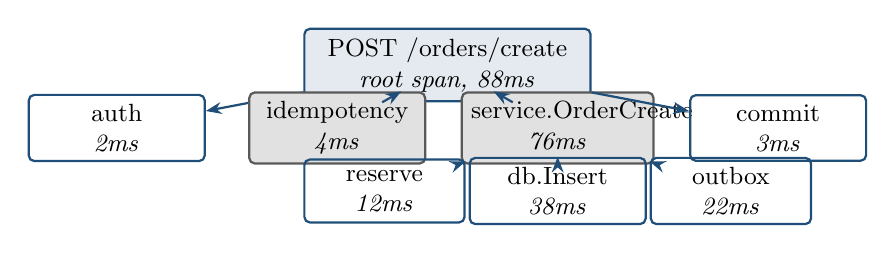
\begin{tikzpicture}[
    every node/.append style={align=center,font=\scriptsize},
    edge from parent/.style={draw=cMain,thick,-{Stealth[length=2mm]}},
    level distance=8mm,
    level 1/.style={sibling distance=28mm},
    level 2/.style={sibling distance=22mm}
  ]
  \node[node-box,node-state-normal,text width=34mm] {POST /orders/create\\\textit{root span, 88ms}}
    child { node[node-box,text width=20mm] {auth\\\textit{2ms}} }
    child { node[node-box,node-state-transition,text width=20mm] {idempotency\\\textit{4ms}} }
    child { node[node-box,node-state-transition,text width=22mm] {service.OrderCreate\\\textit{76ms}}
      child { node[node-box,text width=18mm] {reserve\\\textit{12ms}} }
      child { node[node-box,text width=20mm] {db.Insert\\\textit{38ms}} }
      child { node[node-box,text width=18mm] {outbox\\\textit{22ms}} }
    }
    child { node[node-box,text width=20mm] {commit\\\textit{3ms}} };
\end{tikzpicture}
\vspace{1mm}
\small 一棵树就把"慢在哪一段"答清楚。\textbf{root 88ms} 中 \textbf{db.Insert 占 38ms}，是该接口下一步优化的着力点。
\srcnote{internal/order/service.go OrderCreate 主路径；track.WithSpan 在子函数里开 child span}
\end{frame}

\begin{frame}[fragile]{Jaeger middleware：traceId 透传}
\begin{lstlisting}[language=Go,firstnumber=12,
  caption={\srcnote{middleware/track.go:12--32}}]
func Jaeger() gin.HandlerFunc {
    return func(c *gin.Context) {
        traceId := c.GetHeader("uber-trace-id")
        var span opentracing.Span
        if traceId != "" {
            var err error
            span, err = track.GetParentSpan(
                c.FullPath(), traceId, c.Request.Header)
            if err != nil {
                log.LogrusObj.Warnln(
                    "parse uber-trace-id failed, "+
                    "fallback to local span:", err)
                span = track.StartSpan(
                    opentracing.GlobalTracer(), c.FullPath())
            }
        } else {
            span = track.StartSpan(
                opentracing.GlobalTracer(), c.FullPath())
        }
        defer span.Finish()
        c.Set(consts.SpanCTX,
            opentracing.ContextWithSpan(c, span))
        c.Next()
    }
}
\end{lstlisting}
\end{frame}

\begin{frame}{Jaeger middleware 逐行讲解}
\begin{itemize}
  \item \textbf{第 14 行}：读 \texttt{uber-trace-id} header；格式 \texttt{<traceId>:<spanId>:<parentId>:<flags>}。
  \item \textbf{第 16--18 行}：有 traceId $\to$ 当前请求是别人调过来的，尝试解出上游 context，开 \textbf{child span}，root 留在上游。
  \item \textbf{第 19--23 行}：解析失败时\textbf{不阻断}，打 Warn 日志后退回本地 root span —— header 由客户端控制，畸形头不能拖垮业务请求。
  \item \textbf{第 24--26 行}：没 traceId $\to$ 当前请求是入口，自己开 root span。
  \item \textbf{第 27 行}：\texttt{defer span.Finish()} 必须有，否则 Jaeger 端会看到"未结束"灰色 trace。
  \item \textbf{第 29 行}：把 span 写回 \texttt{c.Context}，下游通过 \texttt{ctl.GetSpanContext} 开 child span —— \textbf{这一步就是"链路"的串接}。
\end{itemize}
\srcnote{pkg/utils/track/track.go:16--33 GetParentSpan Extract}
\end{frame}

\begin{frame}[fragile]{当旁路埋点反噬主链路：畸形 trace 头吞掉整条请求}
\begin{itemize}
  \item \textbf{业务困局}：\texttt{uber-trace-id} 这个 header 由调用方控制 —— 网关透传、客户端拼错、甚至外部扫描器随手塞一个畸形值，都会让 \texttt{GetParentSpan} 的 \texttt{Extract} 解析报错。
  \item \textbf{老写法的陷阱}：解析失败时直接 \texttt{return}，请求\textbf{再也不往下走}。一个本该"旁路"的可观测中间件，把整条业务处理链\textbf{静默吃掉}：用户侧表现为接口无响应/空返回，服务端却\textbf{没有报错日志}，排查时一头雾水。
  \item \textbf{攻击面}：任何人只要发一个非法 \texttt{uber-trace-id}，就能让对应接口\textbf{静默失败}，这是"埋点组件反噬主链路"的典型事故。
\end{itemize}
\begin{lstlisting}[language=Go,firstnumber=19,
  caption={修后（fail-open 降级放行）\srcnote{middleware/track.go:19--23}}]
if err != nil {
    log.LogrusObj.Warnln(
        "parse uber-trace-id failed, "+
        "fallback to local span:", err)
    span = track.StartSpan(
        opentracing.GlobalTracer(), c.FullPath())
}
\end{lstlisting}
\srcnote{middleware/track.go:19--23 解析失败不再裸 return，降级本地 span 后继续 c.Next()}
\end{frame}

\begin{frame}{原则：旁路设施 fail-open，核心链路 fail-closed}
\begin{itemize}
  \item \textbf{旁路设施 fail-open（失败放行）}：埋点、追踪、指标、访问日志这类\textbf{可观测组件}是来"观察"业务的，绝不该成为业务的前置门槛。自身出错时\textbf{降级放行}，最多丢一条 trace，业务照常跑完。
  \item \textbf{核心链路 fail-closed（失败拦截）}：鉴权、限流、风控、库存扣减这类\textbf{安全/一致性关口}，出错或不确定时应\textbf{拒绝} —— 放过的代价是越权、超卖、资损。
  \item \textbf{判断标准}：问"这一层挂了，业务该不该继续？"。可观测层答"继续，留一条 Warn 说明降级"；安全层答"不该继续"。
  \item \textbf{本页修的那行}就是把旁路中间件写成了 fail-closed，等于给系统加了个谁都能触发的隐形开关。
\end{itemize}
\keypoint{中间件的失败语义要和职责对齐：观察类降级放行，守门类拦截兜底。}
\srcnote{middleware/track.go:19--23 fail-open；对照 internal 各 service 校验失败 return 的 fail-closed}
\end{frame}

\begin{frame}{Jaeger 的开销：实测低于 5\%}
\begin{tabular}{@{}lrr@{}}
\toprule
场景 & RPS & p95 \\
\midrule
\texttt{/ping} 裸基线（含 ratelimit/cors/Jaeger 全中间件） & 64{,}254 & 3.51ms \\
\texttt{/product/show} 真业务（MySQL PK + 全中间件）        & 62{,}226 & 3.01ms \\
\bottomrule
\end{tabular}
\vspace{3mm}
\begin{itemize}
  \item \texttt{/ping} 已经过了 \texttt{Jaeger()}（routes/router.go:42 注册），不是"无 trace 裸 RPS"。
  \item 商品详情 RPS 仅比 ping 低 \textbf{3.2\%}，证明全链路 trace 在 const sampler 全量采样下，单机损耗 $<$ 5\%。
  \item 真把损耗摁住，还能从 \texttt{const} 切到 \texttt{probabilistic} 抽样（默认 0.001\%），CPU 占用再降一个数量级。
\end{itemize}
\srcnote{stressTest/REPORT.md 链路压测表第 2、3 行；pkg/utils/track/track.go:15--27 GetDefaultConfig const sampler}
\end{frame}

\begin{frame}{Jaeger 与 Skywalking 同时存在的取舍}
\begin{tabular}{@{}p{2.0cm}p{4.8cm}p{4.0cm}@{}}
\toprule
维度 & Jaeger（OpenTracing） & Skywalking \\
\midrule
插桩方式   & 业务代码显式开 span    & agent 自动织入 \\
学习曲线   & 中（要懂 carrier/inject） & 低（接入即用） \\
定制空间   & 高（可任意标 tag）     & 中（agent 决定） \\
UI / 拓扑 & 单服务 trace 视角     & 全链路服务拓扑图 \\
gomall 用法 & 已落地，主线          & 备选，docker 起着 \\
\bottomrule
\end{tabular}

\medskip
{\small \textbf{业务选型逻辑}：单服务调试用 Jaeger 够细；多服务上线后看拓扑用 Skywalking。两者不冲突，可以并存 —— 当前 gomall 把两套基础设施都备齐，主推 Jaeger，留 Skywalking 做 SRE 大盘。}
\srcnote{cmd/main.go:49 注释掉的 \texttt{//track.InitJaeger()} 留了切换开关}
\end{frame}

% ============================================================
\section{Prometheus 业务 metrics + Grafana 大盘}
% ============================================================

\begin{frame}{SRE 为什么需要 metrics：运营要"实时 GMV 大盘"}
\begin{itemize}
  \item \textbf{业务场景}：双 11 大促 0 点开闸，运营总监站在大屏前盯 GMV 增长曲线；SRE 同时盯下单 p99 和错误率。两边看的是\textbf{同一组指标的不同切面}。
  \item \textbf{运营关心}：当前 RPS、累计 GMV、商家活跃数、转化漏斗（曝光 $\to$ 加购 $\to$ 下单 $\to$ 支付）。$\to$ \texttt{order\_created\_total} + \texttt{paydown\_total} 加业务标签即可呈现。
  \item \textbf{SRE 关心}：下单 p99、错误率、限流命中率、熔断器状态。$\to$ \texttt{order\_create\_duration\_ms} Histogram + \texttt{ratelimit\_hit\_total} + \texttt{circuit\_state}。
  \item \textbf{商家域负责人关心}：商家健康度 —— 平均发货时长、退货率、客诉率。$\to$ 业务指标，从 DB 聚合到 Grafana。
  \item \textbf{业务化设计原则}：指标命名带业务前缀（\texttt{gomall\_order\_*} / \texttt{gomall\_payment\_*}），标签是\textbf{业务语言}（\texttt{status=success/limited/cb\_open}），不是\textbf{技术语言}（\texttt{http\_code=429/503}）。这样运营也能读懂大盘。
\end{itemize}
\srcnote{stressTest/REPORT.md 第 1、4、9 行 RPS / p95 / 错误率三组业务指标在压测期就已经在采}
\end{frame}

\begin{frame}{要给业务接的 4 类 metrics}
\scriptsize
\begin{tabular}{@{}lllll@{}}
\toprule
metric & 类型 & 标签 & 用途 & 来源代码 \\
\midrule
order\_created\_total       & Counter   & status, boss\_id\_bucket  & 单数 / 转化 & internal/order/service.go OrderCreate \\
order\_create\_duration\_ms & Histogram & status                    & p50/p99 & middleware/timing.go（新建） \\
paydown\_total              & Counter   & channel, status           & 渠道占比 & internal/payment/service.go \\
ratelimit\_hit\_total       & Counter   & scope                     & 限流命中率 & middleware/ratelimit.go SlidingWindow \\
circuit\_state              & Gauge     & route                     & 熔断器实时态 & middleware/circuitbreaker.go state \\
idempotency\_hit\_total     & Counter   & route                     & 60002 命中 & middleware/idempotency.go \\
\bottomrule
\end{tabular}
\vspace{2mm}
\small 标签设计原则：\textbf{枚举值数量有限}。\texttt{boss\_id} 不能直接当标签（百万级 cardinality 会把 Prometheus 内存打爆），改成 \texttt{boss\_id\_bucket}（按 GMV 等级分 5 档）。
\srcnote{middleware/ratelimit.go SlidingWindow / middleware/circuitbreaker.go state；指标可在两个中间件里挂}
\end{frame}

\begin{frame}[fragile]{接入 Prometheus：30 行起步}
\begin{lstlisting}[language=Go,firstnumber=1,
  caption={\srcnote{pkg/utils/metrics/metrics.go 草案；与 middleware/timing.go（待建）配合}}]
package metrics

import (
    "github.com/prometheus/client_golang/prometheus"
    "github.com/prometheus/client_golang/prometheus/promauto"
)

var (
    OrderCreatedTotal = promauto.NewCounterVec(
        prometheus.CounterOpts{
            Name: "gomall_order_created_total",
            Help: "订单创建累计计数",
        }, []string{"status", "boss_bucket"})

    OrderDurMs = promauto.NewHistogramVec(
        prometheus.HistogramOpts{
            Name:    "gomall_order_create_duration_ms",
            Help:    "下单耗时（毫秒）",
            Buckets: []float64{5, 10, 25, 50, 100, 250, 500, 1000},
        }, []string{"status"})

    CircuitState = promauto.NewGaugeVec(
        prometheus.GaugeOpts{
            Name: "gomall_circuit_state",
            Help: "熔断器状态 0=Closed 1=Open 2=HalfOpen",
        }, []string{"route"})
)
\end{lstlisting}
\end{frame}

\begin{frame}{Prometheus 接入逐行讲解}
\begin{itemize}
  \item \textbf{promauto 而不是手 Register}：自动注册到默认 Registry，避免漏注册导致 metric 丢失。
  \item \textbf{Counter vs Histogram vs Gauge}：单调递增用 Counter；分位用 Histogram（buckets 是预定义的耗时阈值，决定 p99 精度）；当前态用 Gauge。
  \item \textbf{Histogram buckets 选择}：从 5ms 到 1000ms 八档，参考 \texttt{/orders/create} 实测 p95 $\approx$ 2.3ms（见 deck 10 压测表），5ms 起步刚好覆盖 p95 + p99。
  \item \textbf{标签穷举}：\texttt{status} 取 \texttt{success / fail / limited / cb\_open / idempotent\_hit}，5 个值；\texttt{boss\_bucket} 按 GMV 分 \texttt{S / A / B / C / D}，5 个值。两个标签 5*5=25 个时间序列，可控。
  \item \textbf{怎么暴露}：在 router 加 \texttt{r.GET("/metrics", gin.WrapH(promhttp.Handler()))}，Prometheus 默认 15s 抓一次。
\end{itemize}
\srcnote{Prometheus 官方建议 Counter / Histogram / Gauge 三类用法；stressTest/REPORT.md 第 1--3 行实测 p95 数据}
\end{frame}

\begin{frame}{Grafana 看板：5 个核心面板}
\scriptsize
\begin{tabular}{@{}llll@{}}
\toprule
面板 & 数据源 & 阈值（黄 / 红） & 告警接收人 \\
\midrule
订单总量趋势    & sum(rate(order\_created\_total[5m])) & --- / --- & 不告警 \\
下单 p99 延迟  & histogram\_quantile(0.99, ...) & 200ms / 500ms & SRE \\
下单错误率      & rate(...status="fail"...) / rate(...) & 1\% / 5\% & SRE + 业务 \\
限流命中率      & rate(ratelimit\_hit\_total[1m]) / RPS & 0.5\% / 2\% & SRE \\
熔断器开启次数 & changes(circuit\_state==1[5m]) & 1 次 / 3 次 & SRE + 商家域负责人 \\
\bottomrule
\end{tabular}
\vspace{2mm}
\small \textbf{阈值不是拍脑袋}：基线数据来自压测 —— ping 64K RPS / p95 3.5ms 是\textbf{资源上限}，下单 50K RPS / p95 2.3ms 是\textbf{业务上限}。生产把警戒线放在压测 p95 的 5--10 倍，留出余量。
\srcnote{stressTest/REPORT.md 链路压测表第 1、4 行 p95 数据；阈值倍率参考通用 SRE 实践}
\end{frame}

% ============================================================
\section{ELK / EFK：日志集中化的工程化路线}
% ============================================================

\begin{frame}{客服的"工具盒"：ELK 解决的三类客诉问题}
\begin{itemize}
  \item \textbf{客诉类型 1：用户报"我那笔订单到底有没有出货"} $\to$ 客服在 Kibana 搜 \texttt{userId=10086 AND route="/orders/ship"} $\to$ 看到 5min 前发货 event 已写 outbox $\to$ 答客户"已发，物流单号 SF1234"。
  \item \textbf{客诉类型 2：用户报"我支付的钱去哪了"} $\to$ 搜 \texttt{userId=10086 AND route="/paydown"} 拉时间线 $\to$ 看到 \texttt{status=70002} 熔断 $\to$ 答客户"支付通道刚才异常，已退回，30 分钟内到账"，引用 README 客服话术表。
  \item \textbf{客诉类型 3：商家报"我新上的 SKU 搜不到"} $\to$ 搜 \texttt{level=warn AND msg="ES 不可用"} $\to$ 看到 ES 降级中 $\to$ 答商家"已切到 DB 路径，5 分钟内 ES 恢复就能看到"。
  \item \textbf{所以 ELK 不是"日志收集"}，是\textbf{客服的取证 + 沟通工具}。日志 schema 必须可读：JSON + traceId + userId（脱敏）+ route + status + msg 五件套缺一不可。
  \item \textbf{对应 README 客服话术表}：业务码 70001/70002/50001/60002 + RP-EMPTY 都已经映射到话术，客服从 ELK 看到状态码 $\to$ 直接对照表回话。
\end{itemize}
\srcnote{pkg/utils/log/logger.go logrus；README 业务全景"客服"行：完整业务码表 + 话术}
\end{frame}

\begin{frame}{规模化版本：Filebeat $\to$ Kafka $\to$ Logstash $\to$ ES}
\begin{tikzpicture}[node distance=4mm and 8mm,every node/.append style={align=center,font=\scriptsize,text width=20mm}]
  \node[node-box,node-state-normal]                  (app) {gomall\\N 个实例};
  \node[node-box,node-state-transition,right=of app] (fb)  {Filebeat\\边车 / Daemon};
  \node[node-box,node-state-transition,right=of fb]  (kf)  {Kafka\\log-raw topic};
  \node[node-box,node-state-transition,right=of kf]  (ls)  {Logstash\\过滤 / enrich};
  \node[node-box,node-state-alert,right=of ls]       (es)  {Elasticsearch\\按天分索引};
  \node[node-box,node-state-transition,below=10mm of es] (kb)  {Kibana\\DSL 检索};
  \draw[arrow] (app) -- (fb);
  \draw[arrow] (fb)  -- (kf);
  \draw[arrow] (kf)  -- (ls);
  \draw[arrow] (ls)  -- (es);
  \draw[arrow] (es)  -- (kb);
\end{tikzpicture}
\vspace{1mm}
\begin{itemize}
  \item \textbf{为什么中间加 Kafka}：Filebeat 直连 ES，ES 抖动一次全站日志丢；Kafka 做 buffer，ES 可用性事故不会丢日志。
  \item \textbf{Logstash 做什么}：把 \texttt{traceId} 提取成顶层字段、\texttt{userId} 脱敏（保留前 3 + 后 3 位）、\texttt{level=error} 的同时复制到 \texttt{alert} 索引。
  \item \textbf{按天分索引}：\texttt{gomall-app-2026.05.16}，便于按时间清理（保留 30 天，冷归档到 OSS）。
\end{itemize}
\srcnote{docker-compose.yml:44--99 ES+Kibana 已有；Filebeat/Kafka/Logstash 是路线图}
\end{frame}

\begin{frame}{gomall 启动期的四个 tryInit}
\begin{tikzpicture}[node distance=4mm and 6mm,every node/.append style={align=center,font=\scriptsize,text width=24mm}]
  \node[node-box,node-state-normal] (main) {cmd/main.go\\loading()};
  \node[node-box,node-state-transition,right=18mm of main] (mq)  {tryInitRabbitMQ\\延迟关单不可用};
  \node[node-box,node-state-transition,above=of mq] (es)  {tryInitES\\搜索退回 DB};
  \node[node-box,node-state-transition,below=of mq] (w3)  {tryInitWeb3Listener\\链下监听关闭};
  \node[node-box,node-state-transition,right=of mq] (mv)  {tryInitMilvus\\语义召回关闭};
  \draw[arrow] (main) -- (es);
  \draw[arrow] (main) -- (mq);
  \draw[arrow] (main) -- (w3);
  \draw[arrow-async] (mq) -- (mv);
\end{tikzpicture}
\vspace{2mm}
\begin{itemize}
  \item 四个外部依赖任意一个挂了，HTTP 主路径\textbf{照常起}：登录、浏览、下单、支付都不受影响。
  \item 用户最多失去某一项\textbf{增量能力}：搜不到语义结果、订单不自动延迟关闭，但不会"白屏 500"。
\end{itemize}
\srcnote{cmd/main.go:41, 45--47 调用；:59--102 四个 tryInit 实现}
\end{frame}

\begin{frame}[fragile]{tryInitES：8 行 recover 套路}
\begin{lstlisting}[language=Go,firstnumber=69,
  caption={\srcnote{cmd/main.go:69--78}}]
// tryInitES ES 不可用时静默跳过，搜索接口退回 DB 路径
func tryInitES(ctx context.Context) {
    defer func() {
        if r := recover(); r != nil {
            util.LogrusObj.Warnf("ES 初始化失败，搜索退化: %v", r)
        }
    }()
    es.InitEs()
    initialize.InitSearch(ctx)
}
\end{lstlisting}
\end{frame}

\begin{frame}{tryInitES 逐行讲解：为什么不传 error}
\begin{itemize}
  \item \textbf{第 3--8 行 defer + recover}：底层 \texttt{es.InitEs()} 是\textbf{老代码}，连不上 ES 直接 \texttt{panic}。改 \texttt{InitEs} 签名风险大（连锁影响 search service），所以\textbf{在外层包一个 recover}。
  \item \textbf{为什么不返回 error 让 main 决定}：main 拿到 error 也只能写日志接着启 —— 业务上"ES 挂"和"启动失败"是\textbf{两件事}，前者不应阻塞 HTTP 启动。
  \item \textbf{为什么用 Warnf 不是 Errorf}：error 级别会触发告警；这里是"已知降级路径"，不是异常。给 SRE 留 Warn 让他主动看，不要凌晨 3 点叫人起床。
  \item \textbf{相同套路用了 4 次}：\texttt{tryInitRabbitMQ}、\texttt{tryInitES}、\texttt{tryInitWeb3Listener}、\texttt{tryInitMilvus} —— 同一种姿势，业务上是\textbf{对"不可控外部依赖"的统一回应}。
\end{itemize}
\srcnote{cmd/main.go:59--102 四个 tryInit 同构}
\end{frame}

\begin{frame}{业务码：现有 5 段 + 待加 80xxx 商家段}
\scriptsize
\begin{tabular}{@{}llll@{}}
\toprule
段 & 含义 & 现有 / 新增码 & 客服话术示例 \\
\midrule
20xxx & 业务通用 & ERROR=20001       & "请稍后再试" \\
30xxx & 鉴权     & ErrorAuth*        & "登录已过期" \\
50xxx & 第三方   & ErrorOss=50001    & "上传失败" \\
60xxx & 并发 / 幂等 & 60002 命中     & 静默（用户无感）\\
70xxx & 流量治理 & 70001 限流 / 70002 熔断 & "正在排队 / 当前繁忙" \\
\midrule
80001 & 店铺未审核     & 新增 & "您的店铺还在审核，1--3 工作日" \\
80002 & 操作非本店 SKU & 新增 & "该商品不属于您的店铺" \\
80003 & 提现额度不足   & 新增 & "本月额度已满，下月 1 号刷新" \\
80004 & 发货超时改判即将触发 & 新增 & "您有 N 单超 72h 未发货" \\
80005 & 库存低于阈值   & 新增 & "SKU XXX 库存 $<$ 阈值，请补货" \\
\bottomrule
\end{tabular}
\vspace{1mm}
\small 编码原则同 deck 10：\textbf{HTTP 200 + status 字段}。商家段隔离避免与 admin / C 端文案串号。
\srcnote{pkg/e/code.go 现有 5 段；docs/slides/10-traffic-governance.tex 话术映射模板}
\end{frame}

% ============================================================
\section{静默降级 + SLO + trace 驱动决策}
% ============================================================

\begin{frame}{静默降级的 5 条铁律（提炼自 cmd/main.go 现状）}
\begin{enumerate}
  \item \textbf{依赖必须是"增量能力"}：搜索语义召回、订单延迟关闭、链下事件、消息异步 —— 这些都是"锦上添花"。下单 / 支付 / 鉴权\textbf{不能进降级名单}。
  \item \textbf{兜底路径必须存在}：ES 挂 $\to$ \texttt{InitSearch} 不动，搜索退回 DB \texttt{LIKE \%keyword\%}；Milvus 挂 $\to$ \texttt{semantic-search} 接口短路返回 \texttt{\{items: []\}}。
  \item \textbf{recover 必须配 Warn 日志 + traceId}：不能 silent。"sliently swallow + 0 日志"是事故制造机。
  \item \textbf{recover 范围最小化}：只包 \texttt{InitX}，不包 \texttt{r.Run}。HTTP 主路径要 fail fast。
  \item \textbf{对外可见性}：商家投诉"搜不到我新上的 SKU"时，SRE 一搜 Warn 日志 \texttt{"ES 初始化失败"} 就知道是哪种降级状态。
\end{enumerate}
\srcnote{cmd/main.go:59--102 四个 tryInit 的同构姿势；repository/es/ 退化路径}
\end{frame}

\begin{frame}[fragile]{静默降级的请求期版本：handler 内的弱依赖兜底}
\begin{lstlisting}[language=Go,firstnumber=1,
  caption={\srcnote{service/search/product\_query.go 草案；与 cmd/main.go:70--78 同构}}]
// SearchProducts 弱依赖 ES，主路径返回 DB 结果，
// ES 命中则用 ES 的更优排序覆盖
func (s *ProductSrv) SearchProducts(
    ctx context.Context, kw string) ([]*product.Product, error) {

    // 1. 主路径：DB LIKE，必须返回
    dbResult, err := s.dao.SearchByKeyword(ctx, kw)
    if err != nil { return nil, err }

    // 2. 锦上添花：ES 提供更好的排序
    if !es.Available() {
        log.WithCtx(ctx).Warnf("ES 不可用，搜索降级到 DB")
        return dbResult, nil // 主路径已经够用
    }
    esResult, err := s.esRepo.SearchProducts(ctx, kw)
    if err != nil {
        log.WithCtx(ctx).Warnf("ES 查询出错，降级: %v", err)
        return dbResult, nil
    }
    return mergeResults(dbResult, esResult), nil
}
\end{lstlisting}
\end{frame}

\begin{frame}{请求期降级套路逐行讲解}
\begin{itemize}
  \item \textbf{第 5--6 行}：DB 是\textbf{底盘}，先拿到结果。ES 用还是不用，是优化问题，不是功能问题。
  \item \textbf{第 9--10 行 es.Available()}：bool 缓存上一次健康检查结果（每 5s 更新），避免每次请求都打 ES。
  \item \textbf{第 11 行 log.WithCtx(ctx).Warnf}：traceId 自动注入，客服报"搜不到" $\to$ Kibana 搜 traceId 一眼看清是降级了。
  \item \textbf{第 14--17 行}：ES 报错时\textbf{不 return error}，因为 DB 已经给了答案，用户根本不需要知道 ES 有事。
  \item \textbf{第 18 行 mergeResults}：把 ES 的语义排序 + DB 的 keyword 全量\textbf{融合}，ES 命中段排前，未命中段按 DB 顺序排后 —— 见 deck 21 v2 hybrid 排序。
\end{itemize}
\srcnote{cmd/main.go:70--78 启动期同构；deck 21 v2 hybrid 排序公式}
\end{frame}

\begin{frame}{gomall 的 4 级 SLO 表与年宕预算（与 README 对齐）}
\scriptsize
\begin{tabular}{@{}lllll@{}}
\toprule
SLO 级别 & 例子接口 & 可用率 & 年宕预算 & p99 延迟 \\
\midrule
P0 核心交易 & \texttt{/orders/create} / \texttt{/paydown} & \textbf{99.95\%} & \textbf{4h 22min} & $<$ 500ms \\
P1 核心读   & \texttt{/product/show} / \texttt{/orders/list}   & 99.9\%  & 8h 45min & $<$ 200ms \\
P2 营销秒杀 & \texttt{/coupon/claim} / \texttt{/skill\_product/skill} & 99\%    & 87h 36min & $<$ 200ms \\
P3 信息类   & 轮播 / 分类 / 商家后台 & 99\%    & 87h 36min & $<$ 1s \\
\bottomrule
\end{tabular}
\vspace{1mm}
\begin{itemize}
  \item \textbf{预算思想}：SRE Book 经典 —— "可靠性不是越高越好，多出来的可靠性预算应当转成产品迭代速度"。预算\textbf{是花的}，不是\textbf{省的}。
  \item \textbf{为什么 P0 卡 99.95\% 不卡 99.99\%}：99.99\% 需要多 AZ + 蓝绿 + 主从切换演练，成本翻倍。99.95\% 主从 + Redis + 静默降级即可达到。\textbf{性价比对齐业务体量}。
  \item \textbf{为什么商家后台 P3 = 信息类}：商家可以等、用户不能等。把商家后台从 P0 降到 P3 是\textbf{故意的资源调度}：把 SRE 精力从"半夜修轮播"转移到"白天迭代下单链路"。
  \item \textbf{大促前 budget 预留}：双 11 前一周冻结非紧急上线，把当月剩余 budget 留给大促当天的兜底操作（限流参数微调、熔断阈值微调、强制刷缓存等动作都会"花"预算）。
  \item \textbf{budget 烧完怎么办}：当月剩余 $<$ 50\% $\to$ 冻结非紧急上线；$<$ 20\% $\to$ 冻结所有上线；$<$ 0\% $\to$ 产品 team 全员复盘"为什么 SLO 守不住"。
\end{itemize}
\srcnote{README 业务承诺 SLO 表（P0 99.95\% / P1 99.9\% / P2 99\% / P3 99\%）；Google SRE Book Ch.4}
\end{frame}

\begin{frame}{P0--P3 告警分级与响应 SLA}
\scriptsize
\begin{tabular}{@{}lllll@{}}
\toprule
级别 & 触发条件示例 & 响应 SLA & 通知方式 & on-call 行为 \\
\midrule
P0 & 下单错误率 $>$ 5\%、支付完全不可用 & 5 分钟 & 电话 + IM 全员 & 立即上线，主管同时介入 \\
P1 & 下单 p99 $>$ 1s 持续 10 分钟、ES 全挂 & 15 分钟 & 电话 + IM & 主 on-call 上线 \\
P2 & 限流命中率 $>$ 2\%、熔断器 5 分钟 3 次 & 1 小时 & IM 通知 & 工作时间内排查 \\
P3 & Warn 日志聚集、商家后台慢 & 工作时间 & IM 静默 & 次日复盘 \\
\bottomrule
\end{tabular}

\medskip
\begin{itemize}\setlength{\itemsep}{1pt}
  \item \textbf{分级原则}：不是"看告警严重程度"，是"看用户感知 + 业务收入"。下单挂了影响 GMV，P0；商家后台慢 P3 给 BD 解释一下就行。
  \item \textbf{on-call 轮值}：每周一轮换，工作日 + 周末分两人；P0 双 on-call 自动同时呼叫。
  \item \textbf{post-mortem}：所有 P0 / P1 事故 7 天内必须出 blameless 复盘，沉淀到 wiki。
\end{itemize}

\srcnote{告警阈值与本 deck "Grafana 看板：5 个核心面板" 阈值表对齐}
\end{frame}

\begin{frame}{P0--P3 的业务后果：每一级对应的 GMV 损失}
\scriptsize
\begin{tabular}{@{}llll@{}}
\toprule
级别 & 业务后果 & 估算数字（日 GMV 1000 万） & 客户感知 \\
\midrule
P0 & 全站下单挂、GMV 归零 & \textbf{每 1 min 损失 ~7 千元} & App 弹 "稍后再试"，跳竞品 \\
P1 & 核心读慢、转化率下降 & \textbf{每小时损失 ~5\%} 转化 $\approx$ 2 万元 & 列表转圈，加购流失 \\
P2 & 营销活动慢、ROI 损失 & 单场秒杀少卖 \textbf{10\%--20\%}，营销预算白烧 & 抢券失败客诉，运营道歉 \\
P3 & 信息类慢、体验小问题 & 几乎无 GMV 影响 & 部分用户多等几秒 \\
\bottomrule
\end{tabular}
\vspace{2mm}
\begin{itemize}
  \item \textbf{为什么把 P0 5 分钟卡死}：日 GMV 1000 万 = 每分钟约 7 千元。5min 上线意味着\textbf{单次事故损失上限约 3.5 万元}（不含品牌口碑）。再松就是事故而非降级。
  \item \textbf{为什么 P3 进工作时间}：商家后台慢、运营报表慢，客户感知弱、收入影响小。半夜 3 点叫 SRE 起来修轮播图，是\textbf{SRE 流失制造机}（业内常说"on-call 倦怠")。
  \item \textbf{告警分级 = 业务对故障的真实定价}。不是 P 越多越严肃，是\textbf{把人和钱花在影响最大的事故上}。
\end{itemize}
\srcnote{GMV 估算口径与 README "业务承诺 SLO" P0 99.95\% / P1 99.9\% / P2 99\% / P3 99\% 对齐}
\end{frame}

\begin{frame}{SLO 燃尽预算（Error Budget Burn Rate）}
\begin{itemize}
  \item \textbf{Burn rate} = 当前错误率 $\div$ SLO 允许的错误率。
  \item \texttt{下单 SLO=99.99\%} $\to$ 允许错误率 0.01\%。当前 5 分钟内实测错误率 0.05\% $\to$ burn rate = 5。
  \item \textbf{阈值告警}：
  \begin{itemize}
    \item burn rate $>$ 14.4：1 小时烧完月预算 $\to$ P0
    \item burn rate $>$ 6：6 小时烧完 $\to$ P1
    \item burn rate $>$ 3：1 天烧完 $\to$ P2
    \item burn rate $>$ 1：1 个月烧完（即只是触线）$\to$ P3
  \end{itemize}
  \item \textbf{为什么不用静态阈值}：静态阈值在高峰期容易误报、在低谷期容易漏报；burn rate 是\textbf{相对预算的速率}，跨流量级别都准。
\end{itemize}
\srcnote{Google SRE Workbook Ch.5 Alerting on SLOs 烧穿率告警}
\end{frame}

\begin{frame}{真实案例：从 trace 找到订单列表深分页问题}
\begin{itemize}
  \item \textbf{症状}：商家投诉"翻到第 100 页特别慢"。客服无 traceId 可贴，先用 Kibana 按 \texttt{route: "/orders/list"} 拉日志，发现 90\% 请求耗时 $>$ 5s。
  \item \textbf{用 trace 定位}：在 Jaeger 按 \texttt{op=GET /orders/list} 拉 p99 trace 一条，看到 \textbf{db.Query span 占 root 的 99\%}，扫了 4M 行。
  \item \textbf{优化方案}：游标分页 + Redis 5min 首页缓存（见 PR \#38）。
  \item \textbf{产出效果}：压测对照 —— 旧版 \textbf{8.3 RPS / p95 15.95s}，优化版 \textbf{58{,}406 RPS / p95 5ms}。吞吐 7000x，延迟 3200x。
  \item \textbf{决策闭环}：trace 看出瓶颈 $\to$ PR 优化 $\to$ 压测对比 $\to$ 灰度 $\to$ Grafana 监控 p99 持续观察 1 周。
\end{itemize}
\srcnote{stressTest/REPORT.md 第 8、3 行；PR \#38 游标分页}
\end{frame}

\begin{frame}{业务边界：商家后台 + 可观测不做什么}
\begin{itemize}
  \item \textbf{不做商家自助看板 UI}：BossID API 提供数据，前端\textbf{由商家自己接 Web/App 或对接平台 BI}；招商 pitch 场景用 Postman / Swagger。前端 UI = 独立路线图。
  \item \textbf{不做自定义告警规则}：商家不能自己写"我的销量低于 X 就告警我"。规则由 SRE / 商家域负责人统一维护，避免商家滥用告警把 SRE 拖死。
  \item \textbf{不做日志归档冷存}：当前只保 30 天热索引；7 天以上 OSS 归档 + Glacier 长存是路线图。法务合规口径还没拍板。
  \item \textbf{不做 SaaS 化多商户隔离}：当前 BossID 是\textbf{逻辑隔离}（SQL 加 \texttt{AND boss\_id=?}），不是\textbf{物理隔离}（独立 schema / 独立 RDS）。SaaS 化路线图要再独立讲。
  \item \textbf{不做平台计费 / 抽佣}：商家结算 \texttt{settlement} 表只是聚合，没有真发钱。"按 GMV 抽 5\%" 的财务系统对接由 wallet 服务做（路线图）。
  \item \textbf{不做招商审核流程}：阶段 2--4（OCR / 人工审核 / 试运行）只有文档草案，没有真表 \texttt{merchant\_apply} 和真服务。
  \item \textbf{不做客服工单系统}：客服当前用 ELK + 业务码表 + 话术对照 + 手工 IM 沟通。ticket 表 + 工单 SOP 是路线图。
\end{itemize}
\srcnote{README "业务边界（不做什么）"：没有 merchant role / 没有售后工单 / 没有 SaaS / 不做前端 七条对齐}
\end{frame}

\begin{frame}{五角色共用一套底层信号 + 三件套闭环}
\begin{tikzpicture}[node distance=4mm and 8mm,every node/.append style={align=center,font=\scriptsize,text width=22mm}]
  \node[node-box,node-state-normal]                  (m)   {Metrics\\Prometheus\\发现"有事"};
  \node[node-box,node-state-transition,right=of m]   (t)   {Traces\\Jaeger\\定位"哪一段"};
  \node[node-box,node-state-transition,right=of t]   (l)   {Logs\\Kibana\\看清"什么参数"};
  \node[node-box,node-state-alert,below=8mm of t]    (pr)  {优化 PR\\压测 + 灰度};
  \draw[arrow] (m) -- (t);
  \draw[arrow] (t) -- (l);
  \draw[arrow] (l.south) to[bend right=20] (pr.east);
  \draw[arrow] (pr.west) to[bend right=20] (m.south);
\end{tikzpicture}
\vspace{1mm}
\scriptsize
\begin{tabular}{@{}lll@{}}
\toprule
角色  & 关心的事 & 看哪一层 \\
\midrule
C 端用户 & 我下单成功了吗、钱到哪了 & App 错误码 + traceId（产品提示）\\
商家     & 卖了多少 / 待发几单 / 何时到账 & 商家后台 + settlement（路线图） \\
运营     & 实时 GMV / 商家健康度 & Prometheus + Grafana 业务大盘 \\
客服     & 单个 traceId / 用户做过什么 & Kibana + Jaeger 联查 \\
SRE     & p99 / 错误率 / SLO 预算 / 熔断态 & Grafana + Jaeger + 烧穿告警 \\
\bottomrule
\end{tabular}
\vspace{1mm}
\small 五个角色共用\textbf{同一套信号}（JSON 日志 + trace + Prom 指标），差别只在\textbf{聚合维度}和\textbf{查询入口}。三件套\textbf{缺一不可}：metrics 知道有事不知道在哪、trace 看个体不看趋势、log 看细节不看总体。\textbf{发现 $\to$ 定位 $\to$ 优化 $\to$ 度量}才是真闭环。
\keypoint{可观测性的终态不是工具齐，是\textbf{让业务方独立解释自己的现状} —— 商家解释自己卖得好不好、SRE 解释系统稳不稳、客服解释这一单为什么挂。}
\srcnote{trace + metrics + log 三件套是 SRE/Observability 共识；五角色信号映射与 README "业务全景"对齐}
\end{frame}

% ============================================================
\appendix
% ============================================================

\begin{frame}{面试 Q\&A（1/2）：架构与权限}
\textbf{Q1}：BossID 都在了，为什么不直接给商家开 admin？\\
\hspace{4mm}\small A：admin 看全站数据，商家只能看自店；权限边界不能用"先开放再监控"做。merchant 角色 + \texttt{RequireRole("merchant")} 才是正确解。\textit{[middleware/rbac.go:48--86]}

\vspace{1mm}
\textbf{Q2}：merchant.Group 为什么不在路由层校验 boss\_id？\\
\hspace{4mm}\small A：boss\_id 从 \texttt{ctl.GetUserInfo(ctx).Id} 取，绝不进 body/query。handler 入参故意不暴露该字段 —— "入参里没有 = 没法越权"是设计层面的防御。\textit{[pkg/utils/ctl/ctl.go]}

\vspace{1mm}
\textbf{Q3}：roleCache 为什么 30s 不是 5min？\\
\hspace{4mm}\small A：商家被提权后等 5min 才生效，谈判桌上没法解释。30s 是"权限漂移可接受 + 回源 DB 砍 30 倍"的平衡点；提权时 \texttt{InvalidateRoleCache} 让\textbf{当事人立即生效}。\textit{[middleware/rbac.go:22--45]}

\vspace{1mm}
\textbf{Q4}：商家入驻为什么要先 OCR 再人工审核？\\
\hspace{4mm}\small A：OCR 即时返回，过滤掉资质号不合规、姓名不一致的 80\% 提交，让人工只看真案子。审核 SLA 48h，人工资源精确投放。\textit{[service/ocr.go 待建]}

\vspace{1mm}
\textbf{Q5}：商家看板 4 象限为什么独立加载？\\
\hspace{4mm}\small A：弱依赖契约 —— Redis 挂、库存 ZSET 抖动，不能拖垮整页。每格 2s 独立超时，最差出现"加载中"占位但页面框架不挂。\textit{[与 cmd/main.go:59--102 静默降级同构]}

\vspace{1mm}
\textbf{Q6}：Jaeger 在 64K RPS 下还撑得住吗？\\
\hspace{4mm}\small A：实测 \texttt{/product/show} 全中间件跑 \textbf{62{,}226 RPS}（\texttt{/ping} 64{,}254），开销 $<$ 5\%。const 全量采样压得住；担心损耗可切 probabilistic 0.001\%。\textit{[stressTest/REPORT.md]}
\end{frame}

\begin{frame}{面试 Q\&A（2/2）：可观测性与降级}
\textbf{Q7}：Jaeger 和 Skywalking 同时存在，是不是重复建设？\\
\hspace{4mm}\small A：单服务调试 Jaeger 细，多服务拓扑 Skywalking 直观。两者数据模型相同（trace+span），并存不冲突。gomall 主推 Jaeger，留 Skywalking 做 SRE 大盘。\textit{[cmd/main.go:7]}

\vspace{1mm}
\textbf{Q8}：Prometheus 的 \texttt{boss\_id} 标签为什么不能直接用？\\
\hspace{4mm}\small A：Prometheus 标签 cardinality 必须有限。百万级 boss\_id 会把内存撑爆。改成 \texttt{boss\_bucket}（按 GMV 分 5 档），时间序列数 = 标签笛卡尔积，可控。\textit{[pkg/utils/metrics/metrics.go 草案]}

\vspace{1mm}
\textbf{Q9}：Filebeat 直连 ES 不行吗，为什么还要 Kafka？\\
\hspace{4mm}\small A：Filebeat 直连 $\to$ ES 抖动一次全站日志丢。Kafka 做 buffer，ES 故障期间日志先进 Kafka，恢复后由 Logstash 重放。可用性 $\gg$ 简洁性。\textit{[docker-compose.yml:44--99]}

\vspace{1mm}
\textbf{Q10}：tryInitES 为什么用 recover 不传 error？\\
\hspace{4mm}\small A：底层 \texttt{es.InitEs()} 老代码 panic 风格，改签名牵连大。外层 recover + Warnf 是\textbf{对"启动期不可控依赖"的统一回应}，与请求期熔断（70002）互补。\textit{[cmd/main.go:70--78]}

\vspace{1mm}
\textbf{Q11}：99.99 SLO 怎么落到代码？\\
\hspace{4mm}\small A：burn rate $>$ 14.4 触 P0；下单 / 支付按 P0 配人，商家后台按 P3 配。预算耗尽 50\% 冻结非紧急上线 —— 把可靠性变成 code review 的硬约束。\textit{[Grafana 阈值表对齐]}

\vspace{1mm}
\textbf{Q12}：商家自助接口和 admin 接口业务码段为什么要分？\\
\hspace{4mm}\small A：商家看到的错误码会出现在\textbf{商家 App 文案}里；admin 只在内部后台。两套话术系统不同，业务码隔离段（80xxx vs 20xxx/30xxx）避免文案串号。\textit{[pkg/e/code.go]}
\end{frame}

\begin{frame}[allowframebreaks]{代码位置一览}
\scriptsize
\begin{description}
  \item[BossID 散落字段]\srcnote{internal/order/model.go:14, internal/product/model.go:23, internal/cart/model.go:10, internal/favorite/model.go:17}
  \item[RBAC 中间件]\srcnote{middleware/rbac.go:22--45, :48--86, :89--91}
  \item[Jaeger middleware]\srcnote{middleware/track.go:12--32}
  \item[Trace utility]\srcnote{pkg/utils/track/track.go:16--33}
  \item[Skywalking agent]\srcnote{cmd/main.go:7 import 副作用}
  \item[logrus 初始化]\srcnote{pkg/utils/log/logger.go:14--41}
  \item[静默降级（启动期）]\srcnote{cmd/main.go:59--102 四个 tryInitX 同构}
  \item[静默降级（请求期）]\srcnote{service/search/product\_query.go 草案；deck 21 v2 hybrid}
  \item[merchant.Group 草案]\srcnote{internal/merchant/routes.go 待建，注册进 routes/router.go:58--79 组合根（本 deck p.10）}
  \item[merchant API 7 接口]\srcnote{internal/merchant/handler.go 待建 7 个 handler}
  \item[商家入驻申请]\srcnote{model merchant\_apply (待建)；service/merchant\_apply.go}
  \item[Prometheus metrics]\srcnote{pkg/utils/metrics/metrics.go 草案；middleware/timing.go}
  \item[ELK / EFK 落地]\srcnote{docker-compose.yml:44--99 ES+Kibana；Filebeat/Kafka/Logstash 路线图}
  \item[admin promote 模板]\srcnote{internal/admin/service.go:46--61 PromoteToAdmin}
  \item[admin 路由组]\srcnote{routes/router.go:54--55 admin 组；internal/admin/routes.go:13--15 三接口}
  \item[CircuitBreaker 配置]\srcnote{internal/payment/routes.go:14--21 paydown}
  \item[压测锚点]\srcnote{stressTest/REPORT.md：ping 64{,}254 / product 62{,}226 / 订单优化 58{,}406 vs 旧 8.3 RPS}
\end{description}
\vspace{1mm}
\keypoint{配套：18-merchant-business.tex（商家旅程）/ 10-traffic-governance.tex（流量治理）/ 09 v2 订单状态机 / 13 列表性能 / 21 v2 AI 检索}
\end{frame}

\end{document}
